\section{RESULTS}
\label{sec:hjetscomp:results}

\subsection{Inclusive observables}
\label{sec:hjetscomp:results:inclobs}

\begin{figure}[t!]
  \centering
  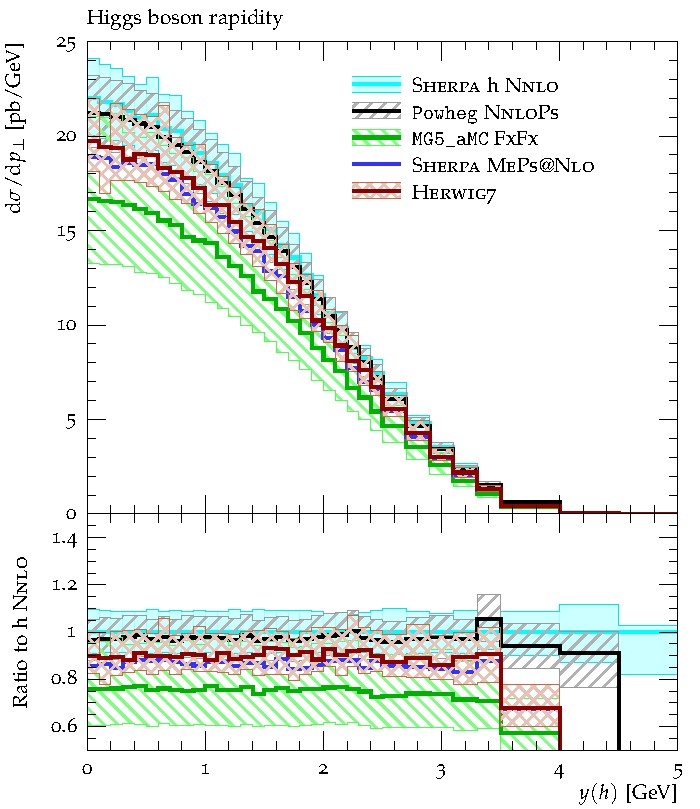
\includegraphics[width=0.47\textwidth]{figures/hjetscomp_H_y.pdf}
  \caption{
    The inclusive Higgs boson rapidity.
    \label{fig:higgscomp:results:inclobs:hy}
  }
\end{figure}

\begin{figure}[t!]
  \centering
  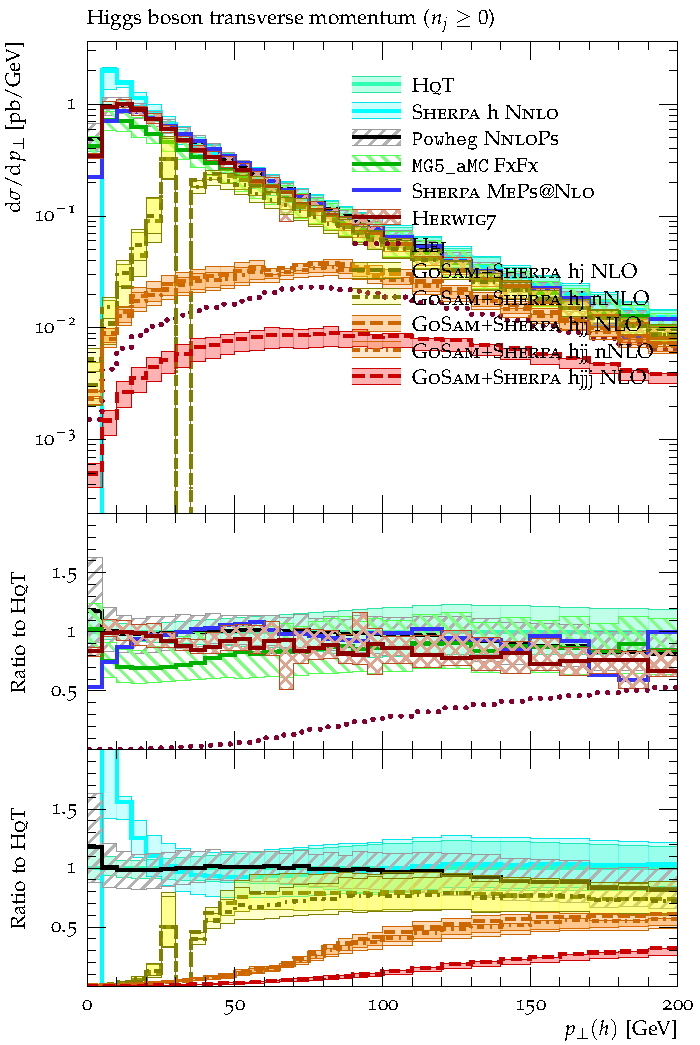
\includegraphics[width=0.47\textwidth]{figures/hjetscomp_H_pT_incl.pdf}
  \quad
  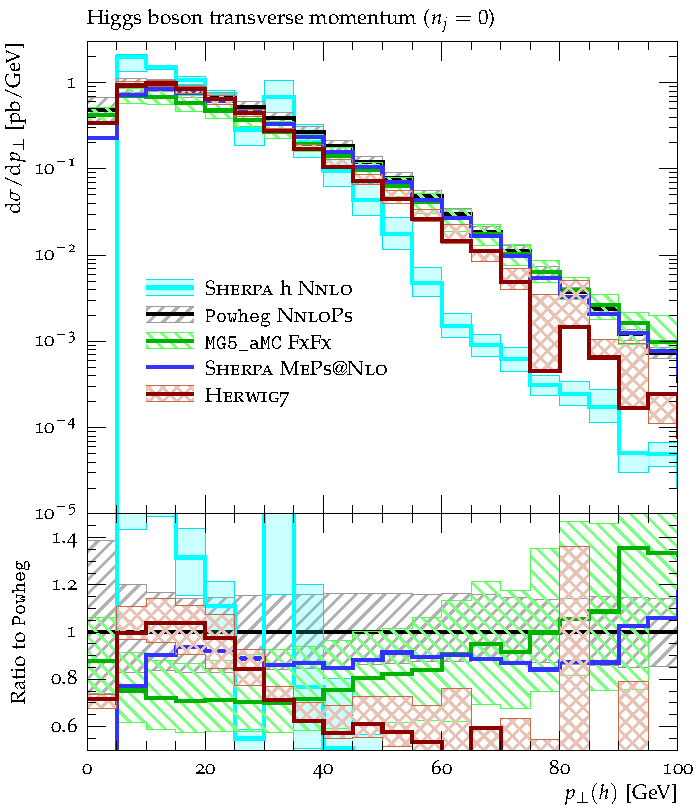
\includegraphics[width=0.47\textwidth]{figures/hjetscomp_H_pT_excl.pdf}
  \caption{
    The Higgs boson transverse momentum in the inclusive event selection 
    (left) and in the absence of any jet (right).
    \label{fig:higgscomp:results:inclobs:hpt}
  }
\end{figure}

\begin{figure}[t!]
  \centering
  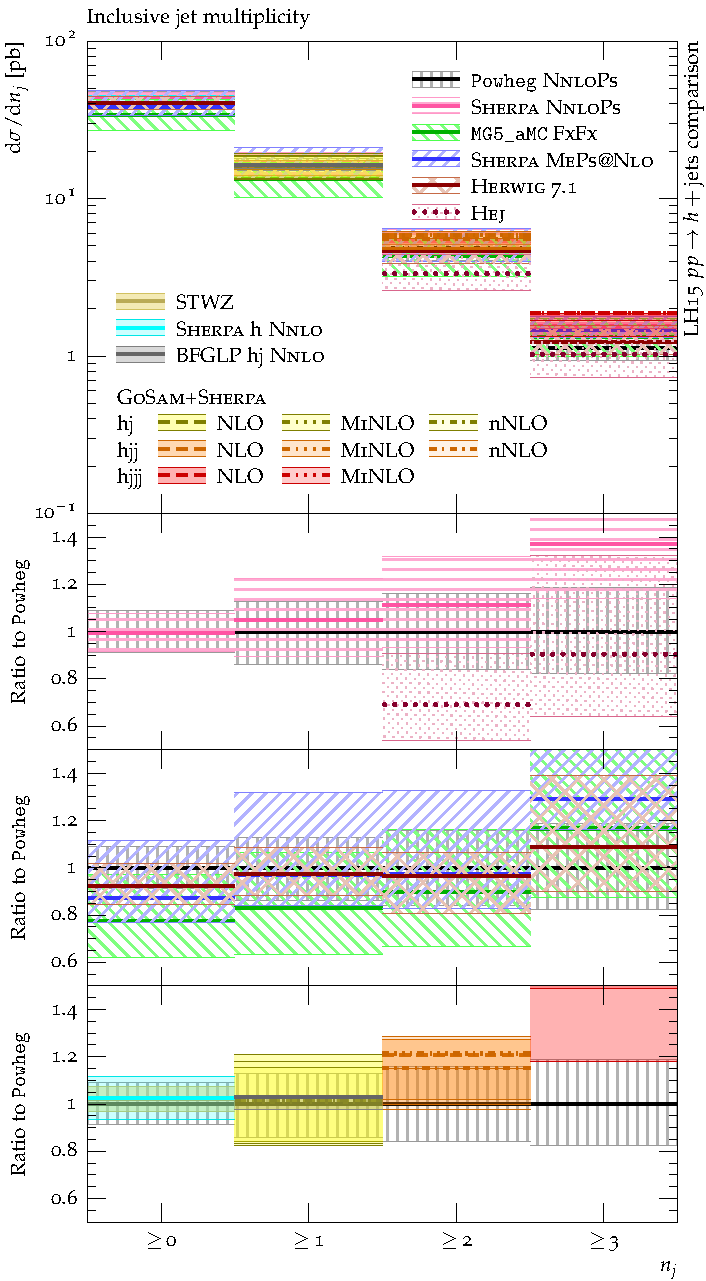
\includegraphics[width=0.47\textwidth]{figures/hjetscomp_NJet_incl_30.pdf}
  \quad
  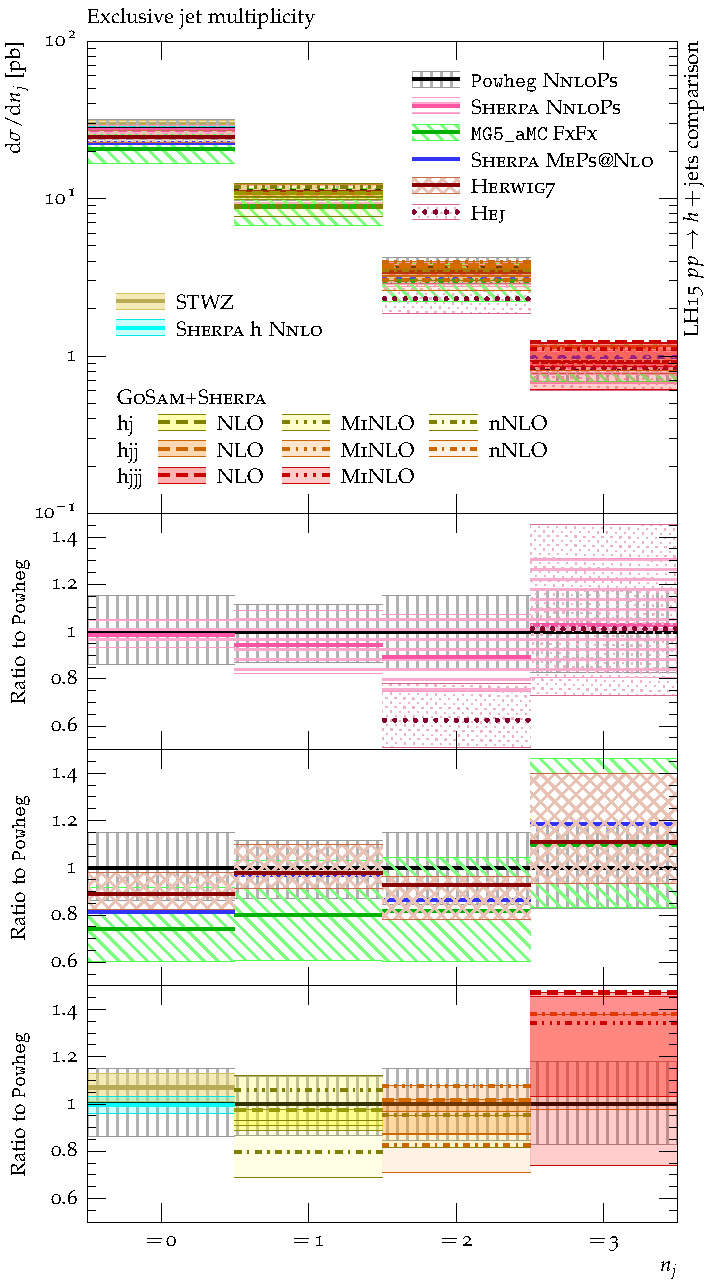
\includegraphics[width=0.47\textwidth]{figures/hjetscomp_NJet_excl_30.pdf}
  \caption{
    The inclusive (left) and exclusive (right) jet multiplicities.
    \label{fig:higgscomp:results:inclobs:njets}
  }
\end{figure}

\subsection{One-jet observables}
\label{sec:hjetscomp:results:1jobs}

\begin{figure}[t!]
  \centering
  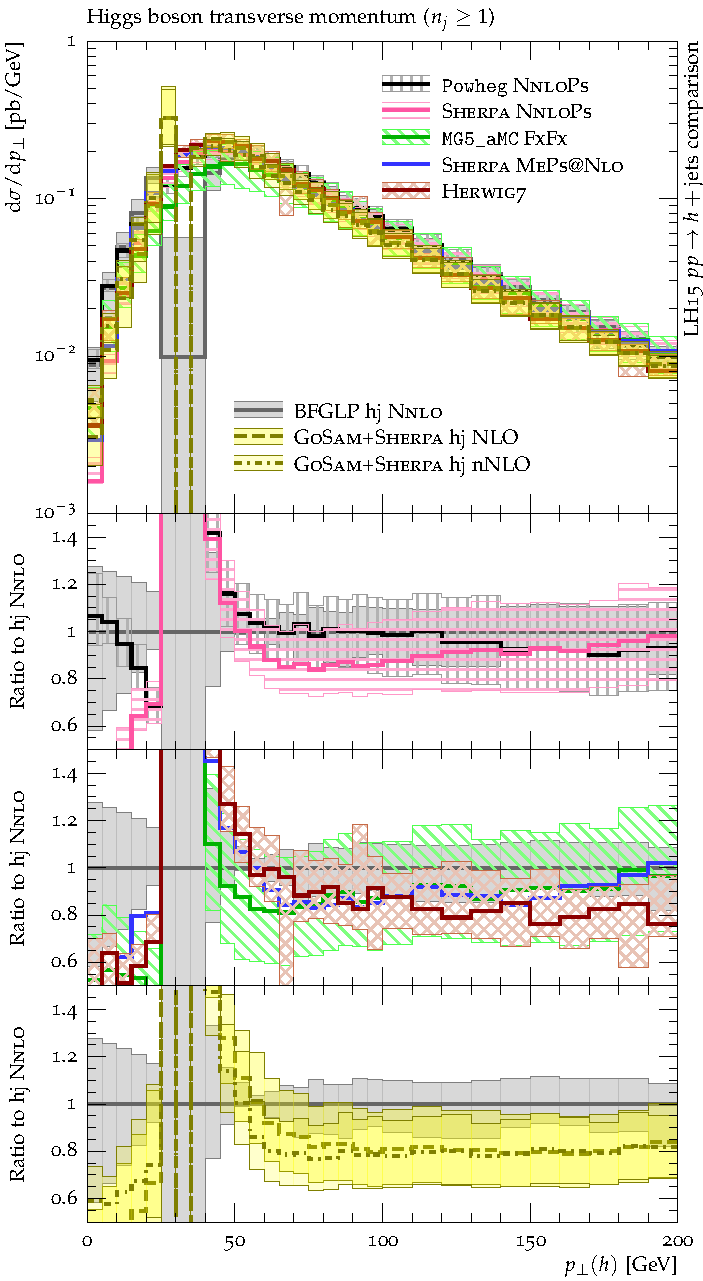
\includegraphics[width=0.47\textwidth]{figures/hjetscomp_H_j_pT_incl.pdf}
  \quad
  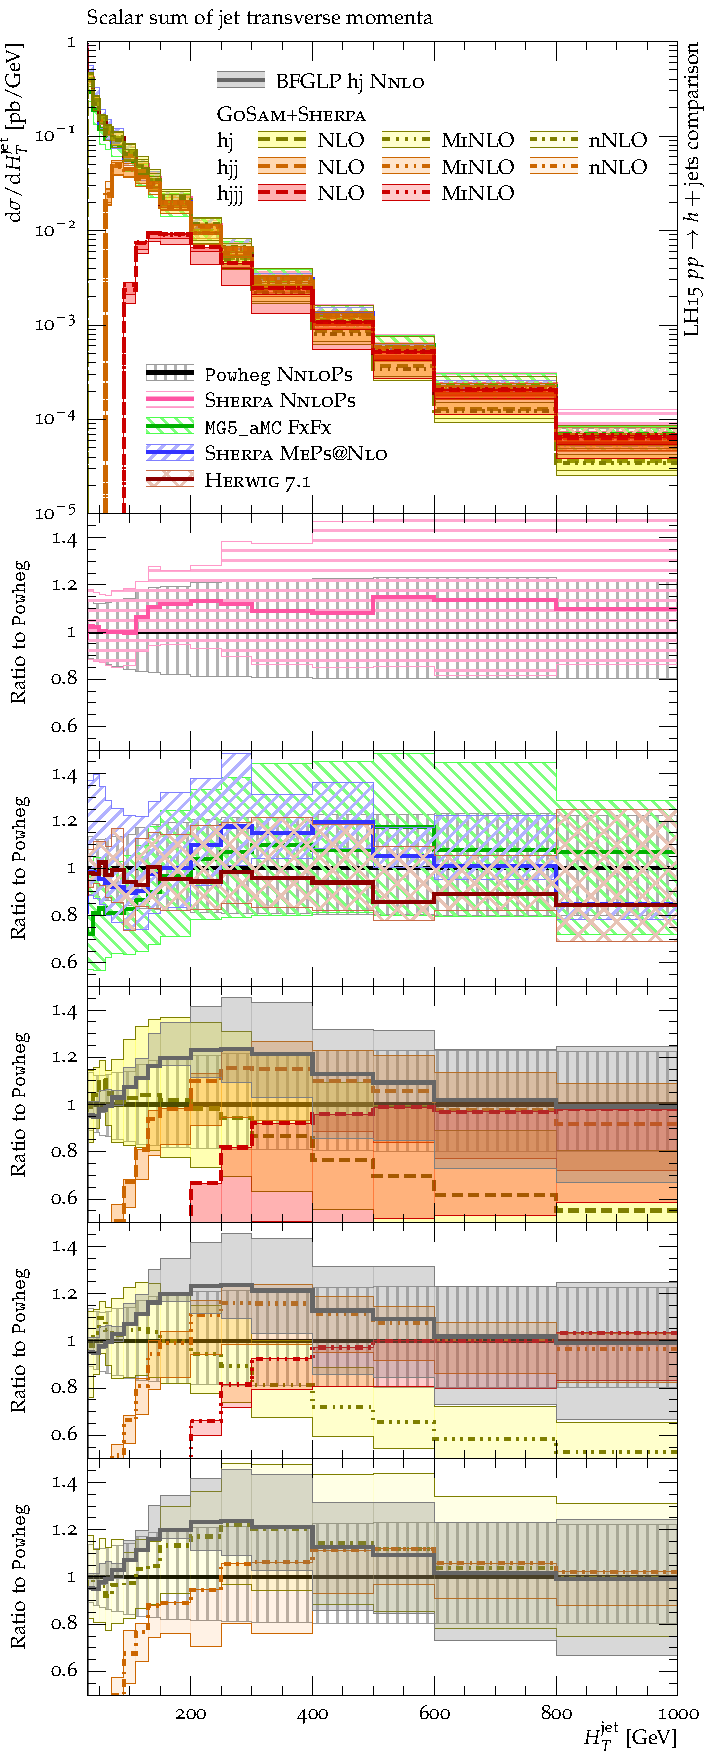
\includegraphics[width=0.47\textwidth]{figures/hjetscomp_HT_jets.pdf}
  \caption{
    The Higgs boson transverse momentum in the presence of at least one 
    jet (left) and in the scalar sum of all jet transverse momenta (right).
    \label{fig:higgscomp:results:1obs:hpt_ht}
  }
\end{figure}

\begin{figure}[t!]
  \centering
  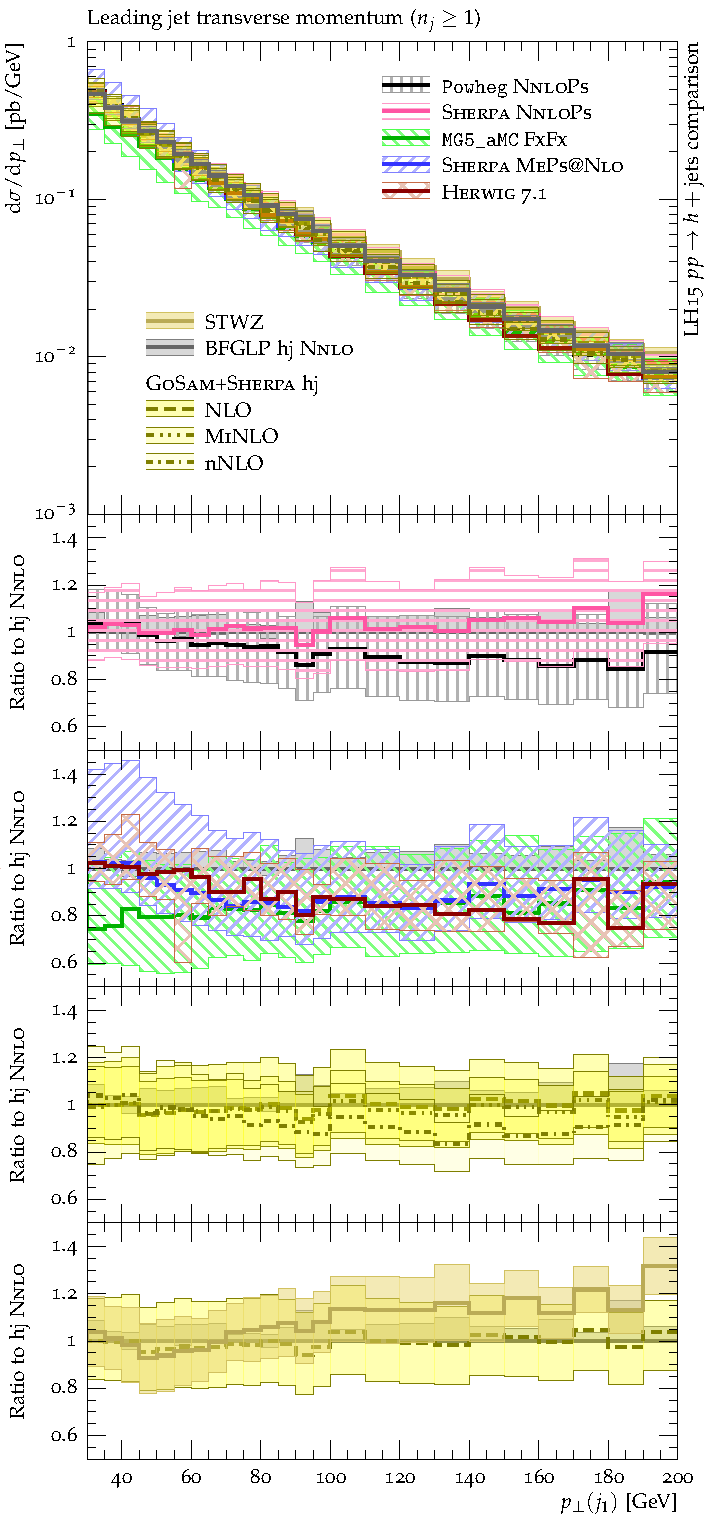
\includegraphics[width=0.47\textwidth]{figures/hjetscomp_jet1_pT_incl.pdf}
  \quad
  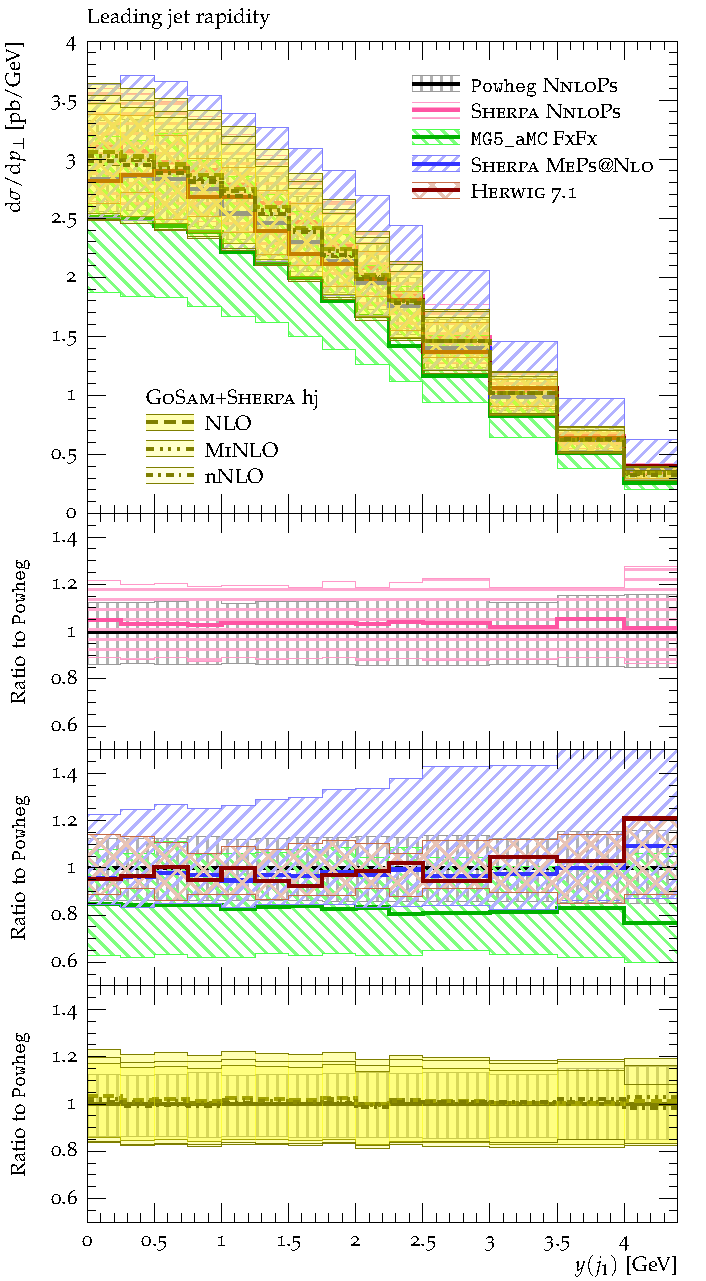
\includegraphics[width=0.47\textwidth]{figures/hjetscomp_jet1_y.pdf}
  \caption{
    The Higgs boson transverse momentum in the presence of at least one 
    jet (left) and in the scalar sum of all jet transverse momenta (right).
    \label{fig:higgscomp:results:1obs:j1pt_j1y}
  }
\end{figure}

\begin{figure}[t!]
  \centering
  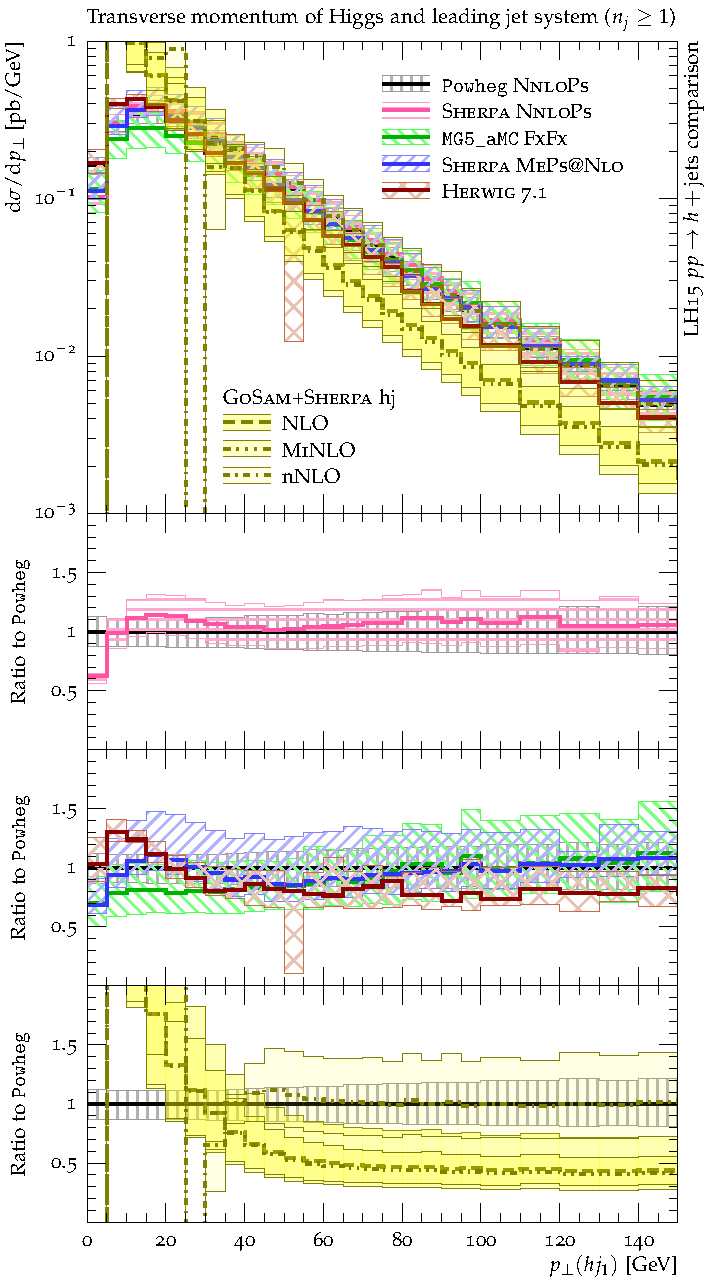
\includegraphics[width=0.47\textwidth]{figures/hjetscomp_Hj_pT_incl.pdf}
  \quad
  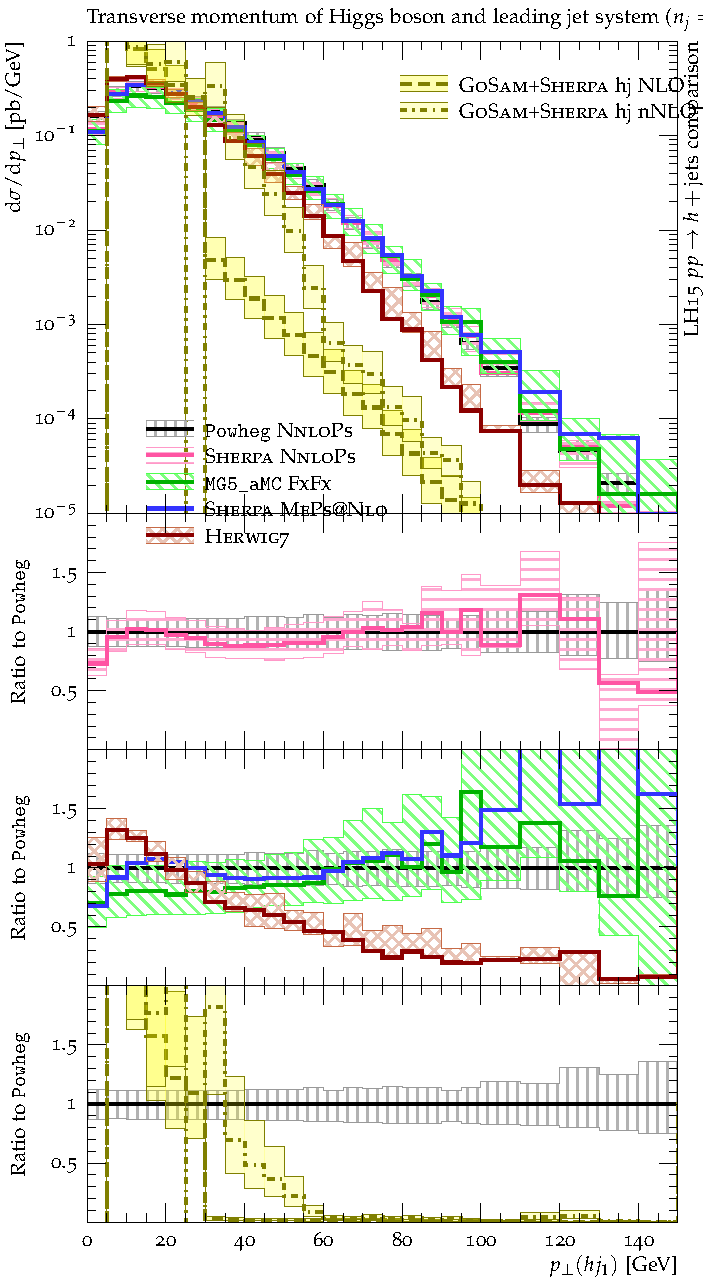
\includegraphics[width=0.47\textwidth]{figures/hjetscomp_Hj_pT_excl.pdf}
  \caption{
    The transverse momentum of the Higgs-boson-leading-jet system in the 
    presence of at least one jet (left) and exactly one jet(right).
    \label{fig:higgscomp:results:1obs:hjpt}
  }
\end{figure}


\subsection{Dijet observables}
\label{sec:hjetscomp:results:2jobs}

\begin{figure}[t!]
  \centering
  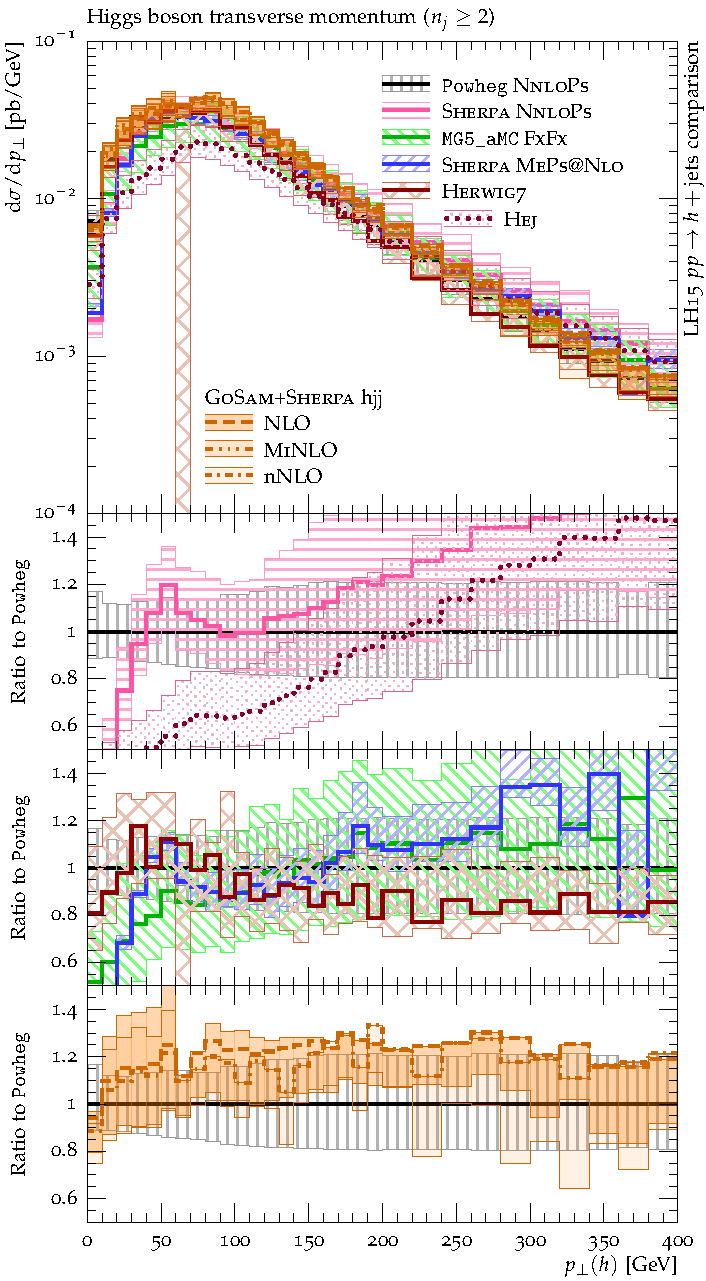
\includegraphics[width=0.47\textwidth]{figures/hjetscomp_H_jj_pT_incl.pdf}
  \quad
  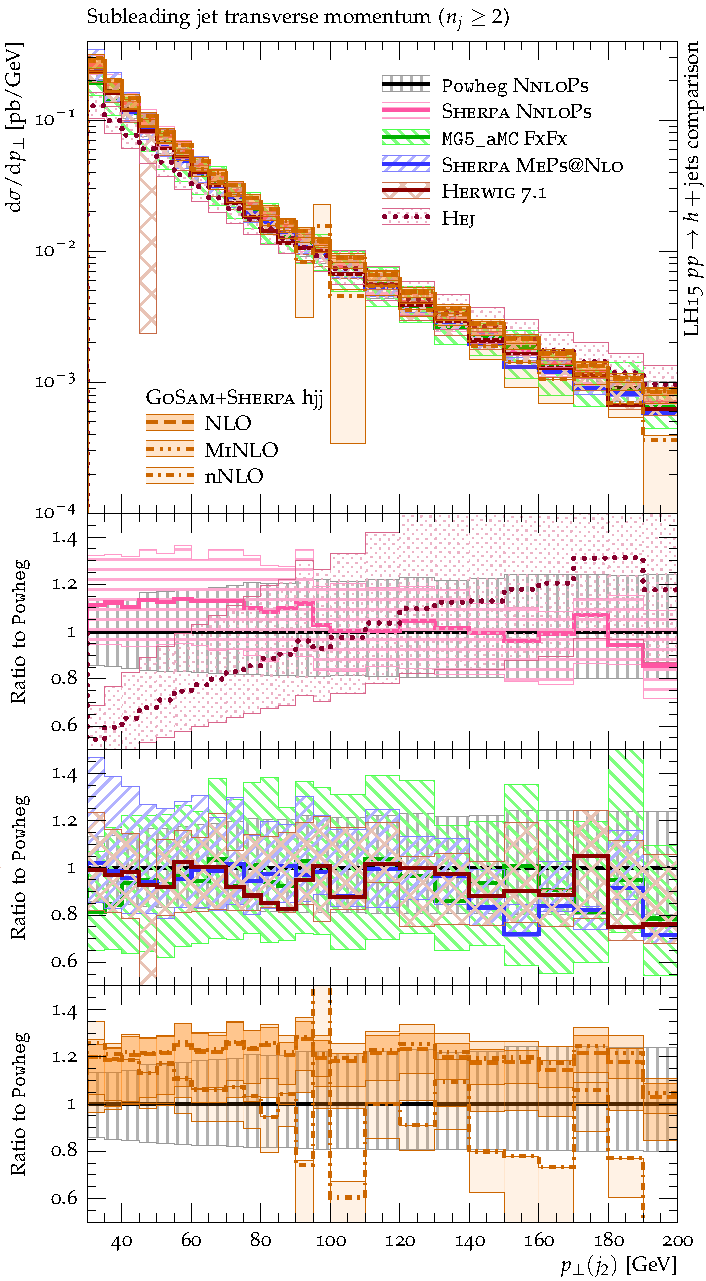
\includegraphics[width=0.47\textwidth]{figures/hjetscomp_jet2_pT_incl.pdf}
  \caption{
    The transverse momentum of the Higgs boson in the 
    presence of at least two jets (left) and the invariant mass of the 
    Higgs boson and the leading dijet system (right).
    \label{fig:higgscomp:results:2obs:hpt_j2pt}
  }
\end{figure}

\begin{figure}[t!]
  \centering
  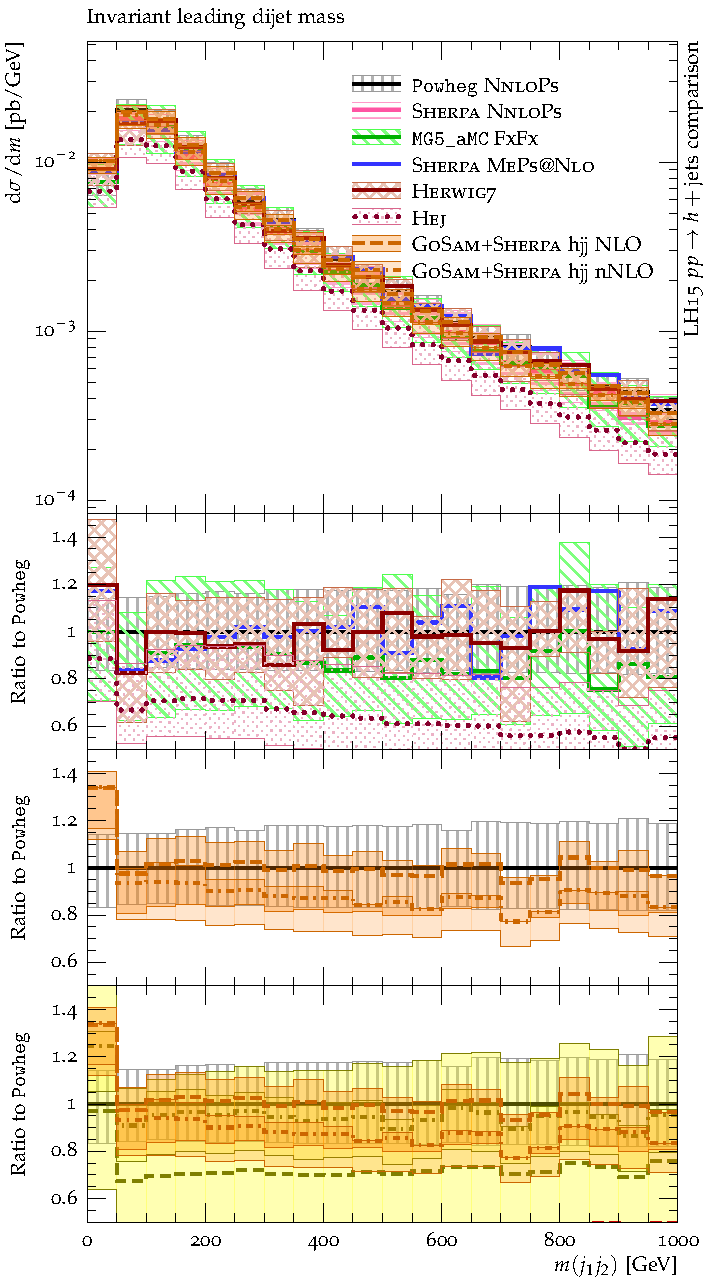
\includegraphics[width=0.47\textwidth]{figures/hjetscomp_dijet_mass.pdf}
  \quad
  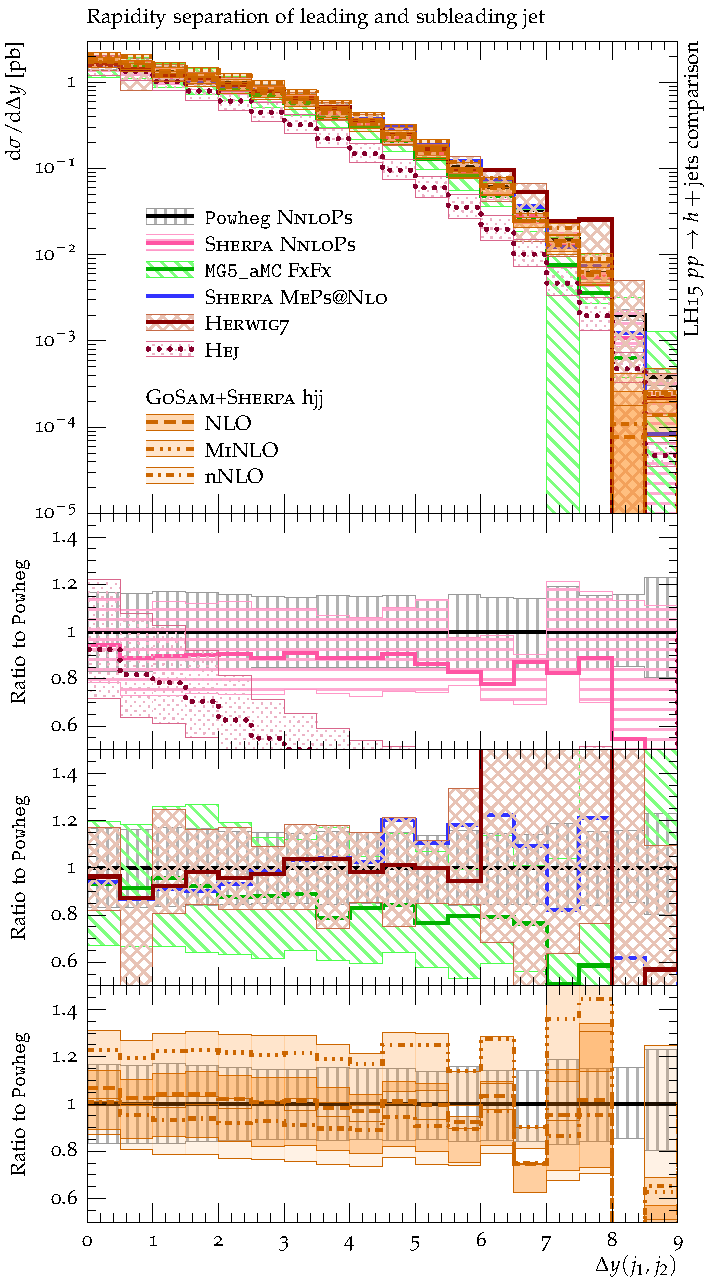
\includegraphics[width=0.47\textwidth]{figures/hjetscomp_deltay_jj.pdf}
  \caption{
    The transverse momentum of the Higgs boson in the 
    presence of at least two jets (left) and the invariant mass of the 
    Higgs boson and the leading dijet system (right).
    \label{fig:higgscomp:results:2obs:mjj_dyjj}
  }
\end{figure}

\subsection{VBF observables}
\label{sec:hjetscomp:results:VBFobs}

\begin{figure}[t!]
  \centering
  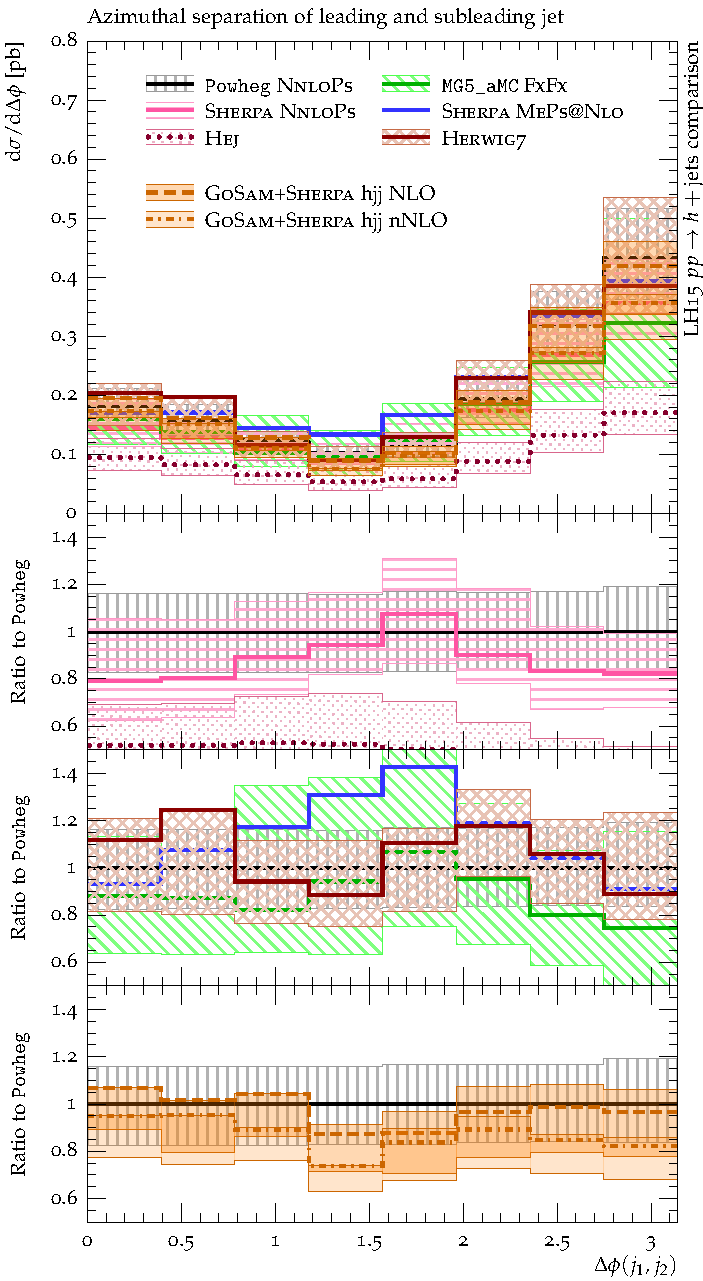
\includegraphics[width=0.47\textwidth]{figures/hjetscomp_deltaphi_jj_VBF.pdf}
  \quad
  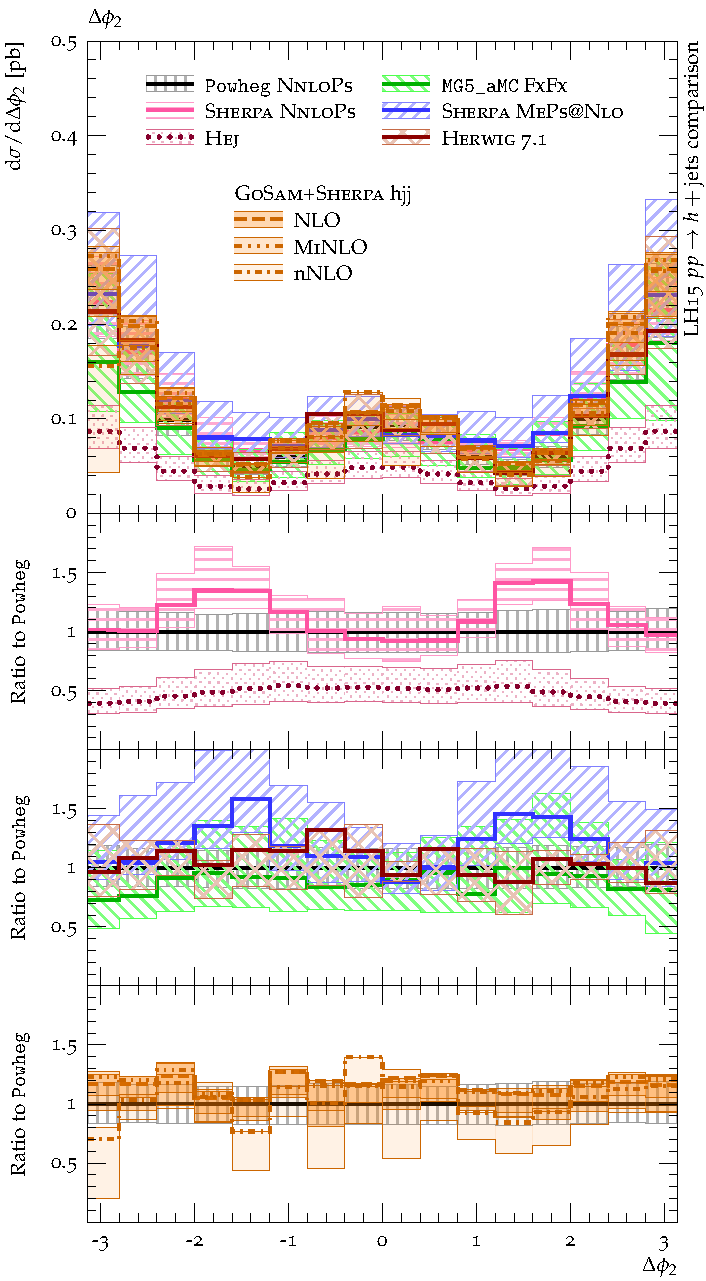
\includegraphics[width=0.47\textwidth]{figures/hjetscomp_deltaphi2_VBF.pdf}
  \caption{
    Azimuthal separation of the leading jet pair (left) and 
    $\Delta\phi_2$ (right) after applying VBF cuts.
    \label{fig:higgscomp:results:VBFobs:dphijj_phi2}
  }
\end{figure}




\subsection{Multijet observables}
\label{sec:hjetscomp:results:mjobs}

\begin{figure}[t!]
  \centering
  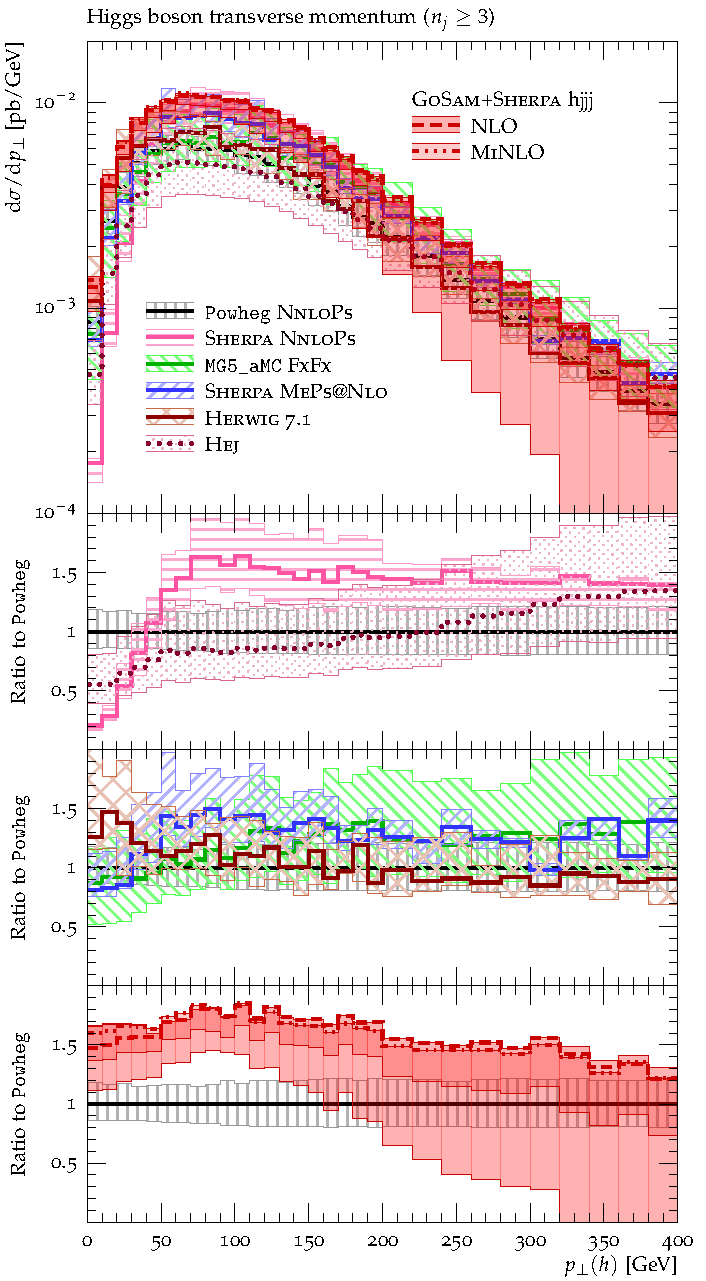
\includegraphics[width=0.47\textwidth]{figures/hjetscomp_H_jjj_pT_incl.pdf}
  \quad
  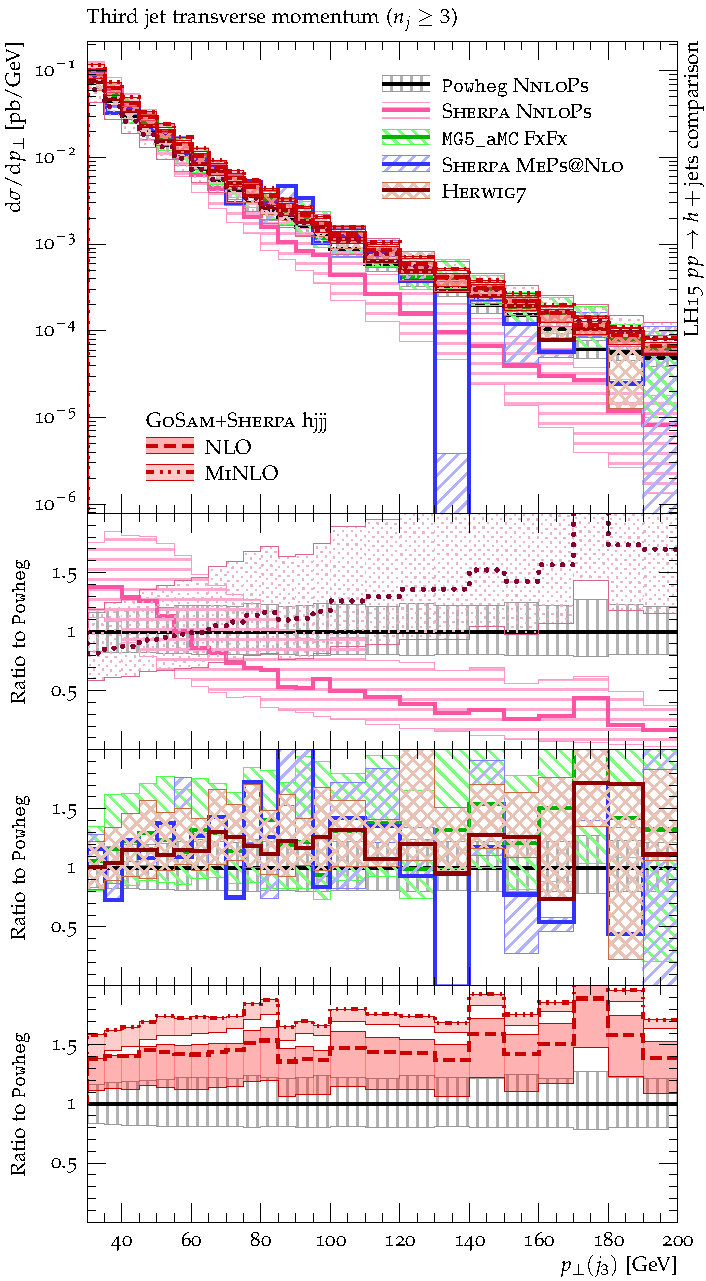
\includegraphics[width=0.47\textwidth]{figures/hjetscomp_jet3_pT_incl.pdf}
  \caption{
    The Higgs boson transverse momentum in the presence of at least three 
    jets (left) and transverse momentum of the third jet (right).
    \label{fig:higgscomp:results:mobs:hpt_j3pt}
  }
\end{figure}

\subsection{Jet veto observables}
\label{sec:hjetscomp:results:jvobs}

\begin{figure}[t!]
  \centering
  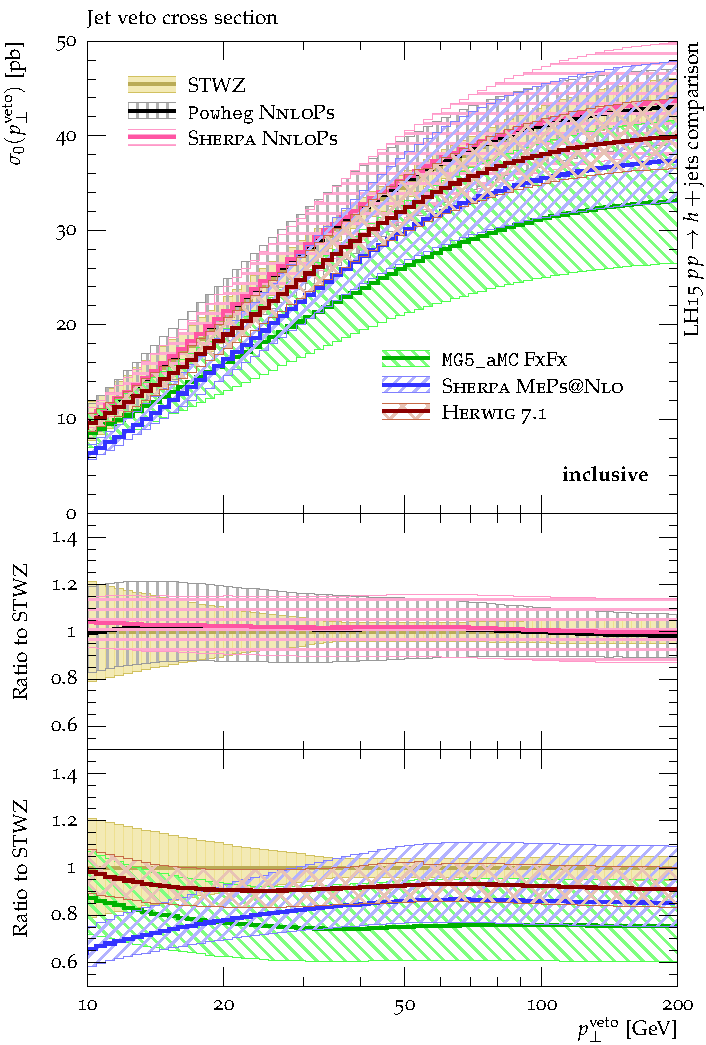
\includegraphics[width=0.47\textwidth]{figures/hjetscomp_xs_jet_veto_j0.pdf}
  \caption{
    Exclusive zero jet cross section in dependence on the vetoed minimal 
    leading jet transverse momentum.
    \label{fig:higgscomp:results:jvobs:jvxs0}
  }
\end{figure}


\begin{figure}[t!]
  \centering
  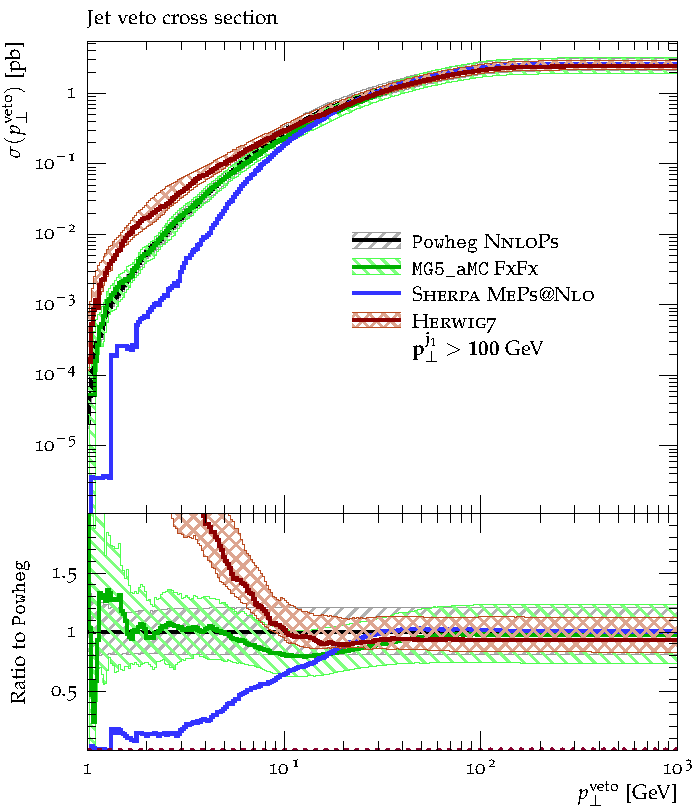
\includegraphics[width=0.47\textwidth]{figures/hjetscomp_xs_jet_veto_j1_100.pdf}
  \quad
  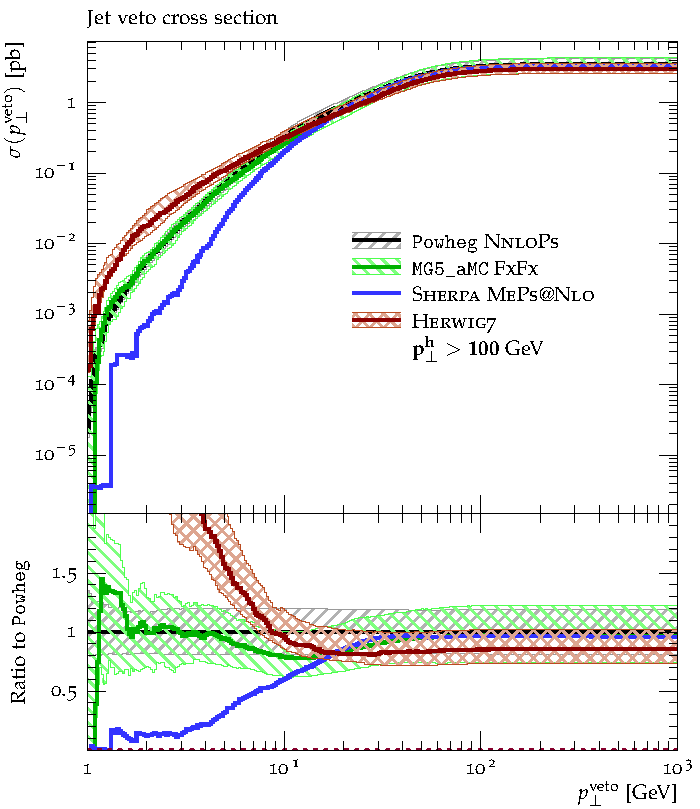
\includegraphics[width=0.47\textwidth]{figures/hjetscomp_xs_jet_veto_h_100.pdf}
  \caption{
    Cross section of events with a Higgs boson (left) or a leading jet (right)
    with a transverse momentum of at least 100 GeV in dependence on the 
    vetoed minimal subleading jet transverse momentum.
    \label{fig:higgscomp:results:1obs:jvxs1h_jvxs1j}
  }
\end{figure}

\begin{figure}[t!]
  \centering
  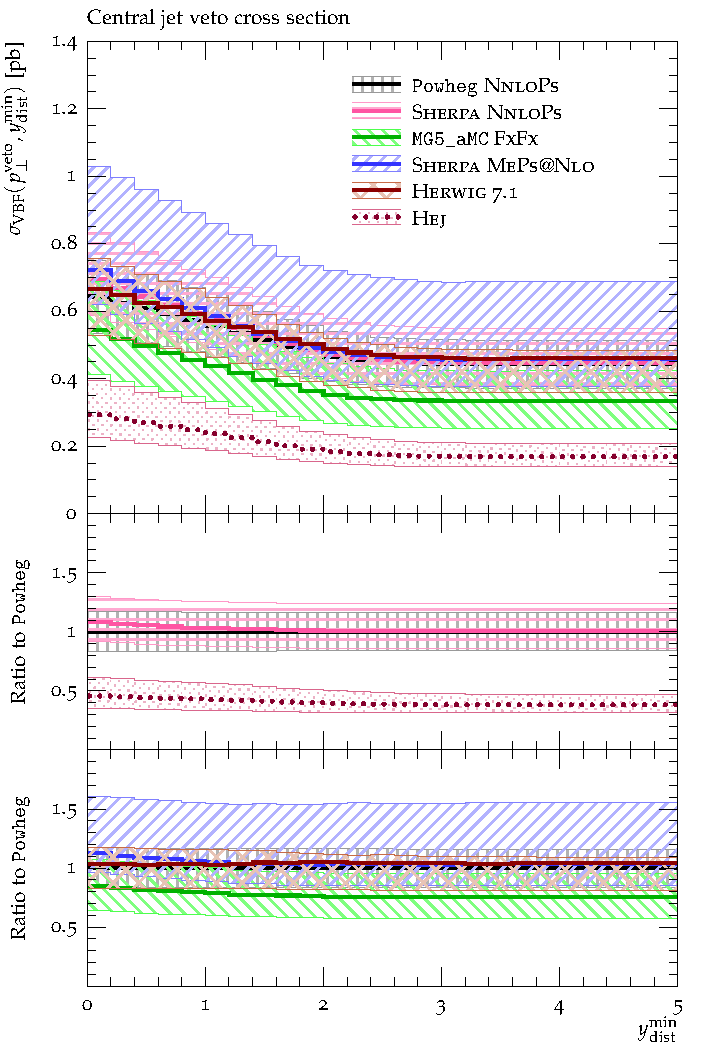
\includegraphics[width=0.47\textwidth]{figures/hjetscomp_xs_central_jet_veto_VBF.pdf}
  \caption{
    Cross section after VBF cuts in dependence with the veto on the leading 
    central jet with transverse momentum larger than 30 GeV in dependence 
    of the rapidity distance of the tagging jets.
    \label{fig:higgscomp:results:1obs:cjvxsvbf}
  }
\end{figure}

